\documentclass[]{rsos}

\begin{document}

\title{Survival depends critically on predator detection in zebrafish larvae}

\author{%%%% Author details
Arjun Nair, Christy Nguyen, and Matthew J. McHenry}

%%%%%%%%% Insert author address here
\address{Department of Ecology and Evolutionary Biology\\
University of California, Irvine\\
321 Steinhaus Hall\\
Irvine, CA 92697}

\title{Supplemental figures}

% This is the code to put the 'S' in front of the figure numbers
\setcounter{figure}{0}
\renewcommand{\thefigure}{S\arabic{figure}}%

\begin{figure}[!h]
\centering
	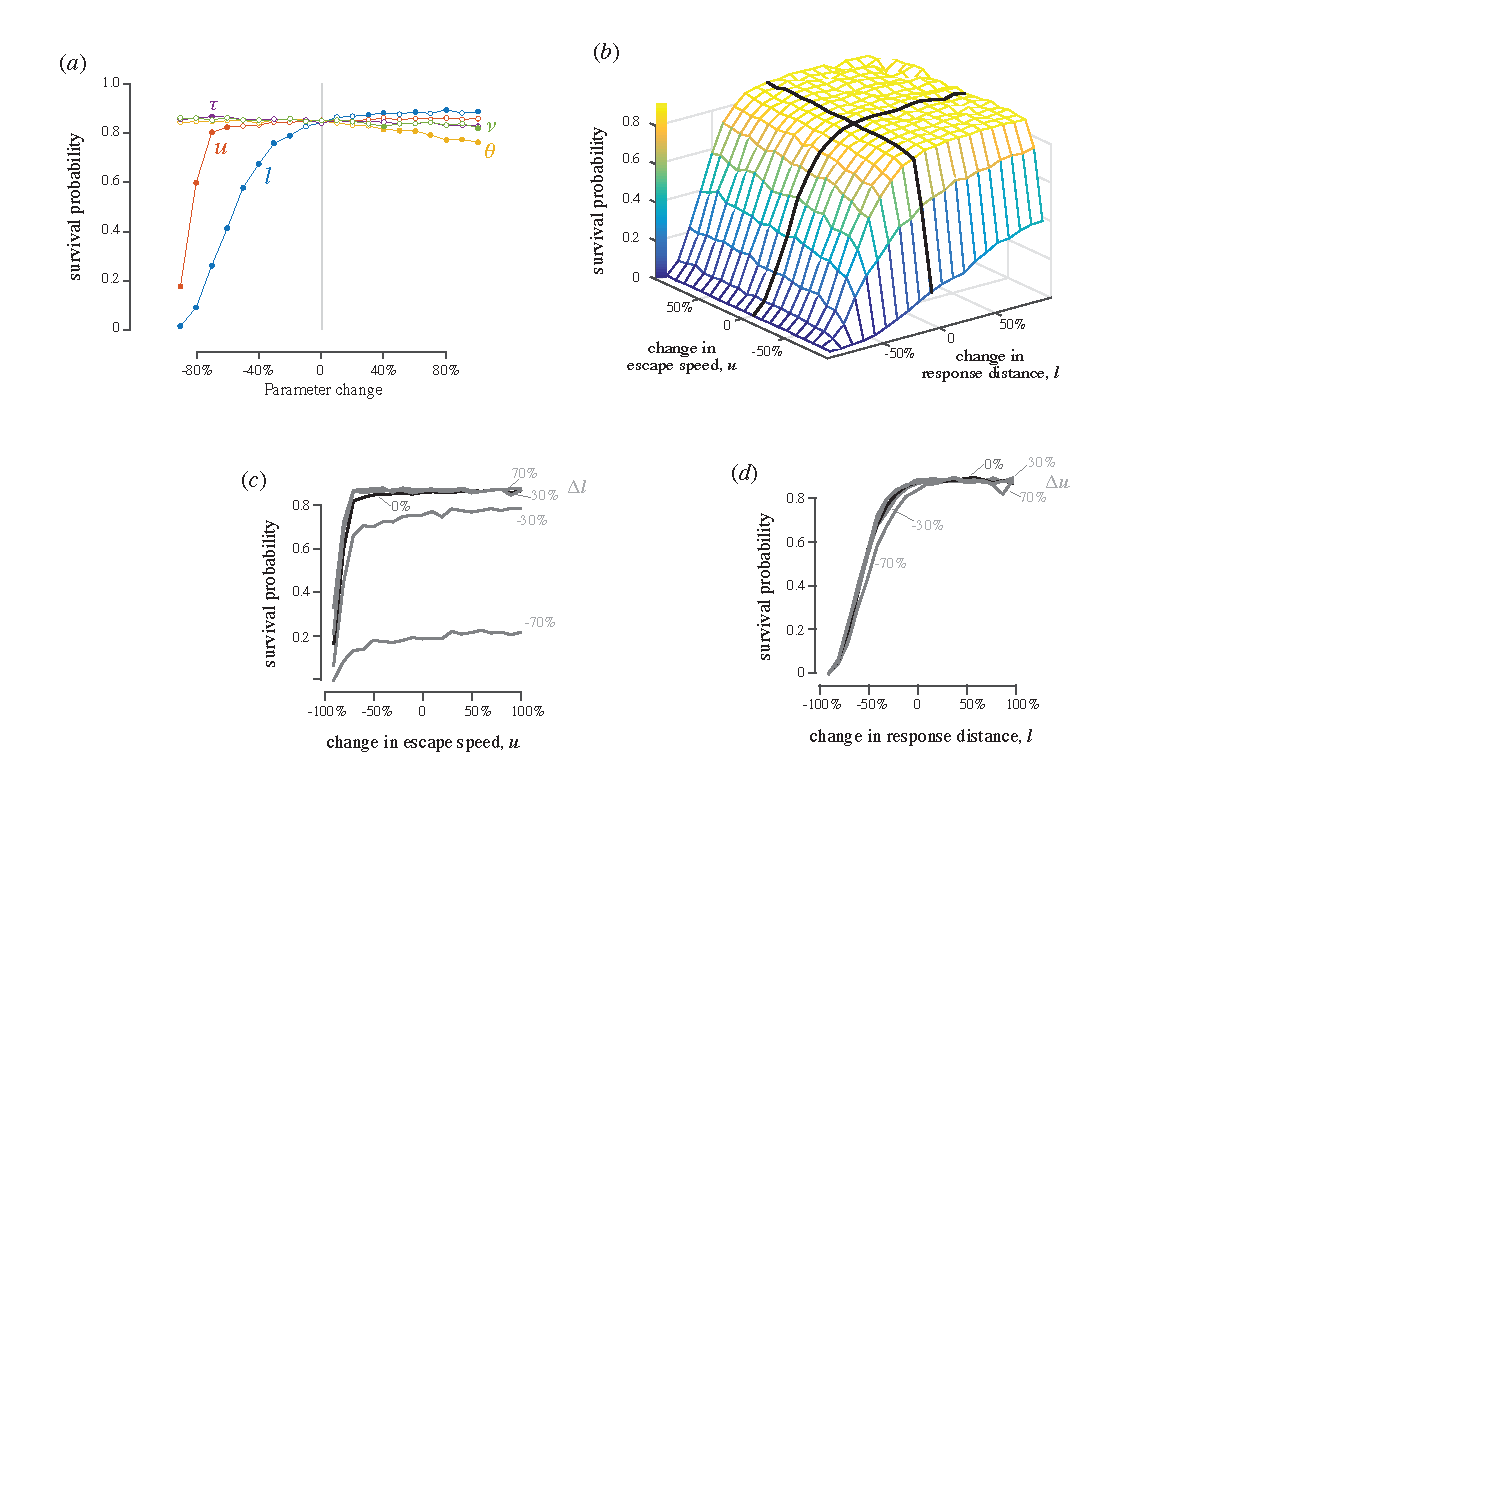
\includegraphics[width=5.5in]{supp_fig_sensitivity}
\caption{Sensitivity analysis of game model to examine the effects of parameter variation on escape probability for juvenile zebrafish. 
(\textit{a}) Varying the the mean of the distribution by manipulating the log-mean value (see Table 1 in main manuscript for parameter definitions and values), with each point representing the result of 1000 simulations. 
(\textit{b}) Variation in escape probability was examined with respect to both escape speed and response distance the same simulation results are shown with respect to changes in escape speed (\textit{c}) and response distance (\textit{d}).
}
\label{supp_fig_sense}
\end{figure}

\end{document}